% =====================================================================
%  When Drift Breaks: Particle-Based Regime Inference for Crash Detection
%  main_v16.tex
%
%  Rekonstruiert aus paper1_v15_revised.pdf (Loge, 23. Mai 2026, Lijiang).
%  Die LaTeX-Quelle zu v14/v15 war verloren; diese Datei ist die
%  wiederhergestellte Quelle, mit drei inhaltlichen Korrekturen
%  gegenueber v15 (siehe % KORREKTUR-Markierungen).
%
%  Abbildungen: figure1_precursors.pdf und figure2_separation.pdf,
%  extrahiert aus dem Figures-Companion-PDF (Vektorgrafik). Fuer die
%  finale Einreichung idealerweise durch die matplotlib-Originale
%  (hoechste Aufloesung) ersetzen, falls auffindbar.
%
%  Dokumentklasse: Standard-article. Die Original-Journal-Klasse
%  (vermutlich interact.cls) ging aus dem PDF nicht hervor; fuer die
%  Reviewer-Version vor Einreichung ggf. auf die QF-Klasse umstellen.
% =====================================================================
\documentclass[11pt]{article}

\usepackage[utf8]{inputenc}
\usepackage[T1]{fontenc}
\usepackage[margin=2.5cm]{geometry}
\usepackage{amsmath,amssymb}
\usepackage{graphicx}
\usepackage{booktabs}
\usepackage{natbib}
\usepackage{caption}
\usepackage[hidelinks]{hyperref}

\bibliographystyle{plainnat}

\setlength{\parindent}{1.2em}
\setlength{\parskip}{0.3em}

% --- Titel -----------------------------------------------------------
\title{When Drift Breaks: \\
       Particle-Based Regime Inference for Crash Detection}

\author{Lutz Pl\"umer\\
  \small University of Bonn, Germany (Emeritus);\\
  \small Southwest Jiaotong University, Chengdu, P.R. China}

\date{}

% =====================================================================
\begin{document}
\maketitle

% --- Abstract --------------------------------------------------------
\begin{abstract}
Whereas existing approaches to financial regime detection work by
recognition---identifying crises through their resemblance to past
episodes---we propose a framework built on immunization: a particle
filter whose observation model is calibrated to the distributional
shape of market stress rather than to the specific characteristics of
historical crisis episodes. The particle filter, whose theoretical
foundations were established in probabilistic robotics and modern
autonomous driving \citep{Thrun2005} and recently applied to financial
markets by Biswas, Reisinger et al.\ (2023), forms the inferential
backbone of our framework. The observation model consists of a novel
combination of this particle filter with a detailed multi-scale
observation model: a stack of distributional shape descriptors---
skewness, tail asymmetry, kurtosis, and the share of leading
sector-eigenvalue energy in cross-asset return covariance---computed
across a hierarchy of temporal windows and transferred to the filter as
structured distributional archetypes through strategic particle
injection, replacing the random initialization of both Thrun et al.\ and
Reisinger et al. Applied to S\&P~500 data across four structurally
distinct crisis episodes (Dotcom 2002, Lehman 2009, COVID-19 2020, and
the inflation-driven bear market of 2022), the framework's
distributional shape descriptors demonstrate consistent pre-crisis
discrimination, with effect sizes (Cohen's $d$) exceeding 2.9 for
realized volatility, Bowley downside skewness, and tail quantile
features, and exceeding 1.3 for the sector concentration feature
($\lambda_1$ ratio) across all four crises. On out-of-sample test data
(2015--2026), the pipeline reports remarkable lead times before
classical momentum indicators for endogenous regime transitions, while
correctly classifying the 2025 Hormuz episode as a Bear regime rather
than a Crisis, consistent with its eventual peak-to-trough drawdown of
approximately 19\%. The results support a single claim: in the context
of particle filters, the richness of the observation model is the
primary enabler of early regime detection. We therefore propose to
direct research efforts towards the construction of a new class of
indicators and oscillators specifically designed for the early
detection of regime changes.

\medskip
\noindent\textbf{Keywords:} regime detection; particle filters;
distributional shape; higher-order moments; early warning systems;
financial crises
\end{abstract}

% =====================================================================
\section{Introduction}

Financial markets are not stationary systems in a statistical sense---
but their regimes, to a significant extent, are. Within a sustained Bull
market, the statistical properties of log daily returns are
approximately stable: volatility is low, the return distribution is
mildly positively skewed, and the tails are thin. Within a Crisis
regime, a different stationarity prevails: volatility is high, skewness
turns sharply negative, and the tails are fat. What is not stationary at
all is the transition between these states.

This observation---that regimes differ not only in their first and
second moments but in their higher-order distributional structure,
including skewness, kurtosis, and tail asymmetry---is the point of
departure for this paper. Regime transitions are both practically
relevant and theoretically challenging precisely because they violate
the assumptions that make standard models tractable: Gaussianity,
homogeneity of variance, and the stationarity of the data-generating
process. Crashes represent the extreme case. As Biswas, Reisinger et
al.\ (2023) demonstrate in their treatment of interacting particle
systems and McKean-Vlasov SDEs with non-differentiable drift
coefficients, the collective dynamics of financial markets near a crisis
episode are characterised by a breakdown of the regularity assumptions
that underpin standard numerical methods---a regime in which the drift
is no longer differentiable and classical econometric models fail
precisely when they are most needed.

While Thrun et al.\ provide our methodological foundation, and Biswas,
Reisinger et al.\ demonstrate the relevance of particle-based methods in
non-smooth financial contexts, within the framework of particle filters,
our key innovation lies in multi-scale distributional shape analysis.
Rather than monitoring point estimates or summary statistics, we track
the evolution of entire return distributions across multiple time
horizons. This approach reveals subtle structural changes that precede
obvious price movements, enabling early detection of regime transitions.
The methodology draws inspiration from Scale-Invariant Feature Transform
(SIFT) techniques in computer vision \citep{Lowe2004}, adapting the
multi-scale analysis paradigm to financial time series.

What makes this particular approach unique is the departure from random
particle injection---the standard solution in both Thrun's robotics
framework and Reisinger's financial formulation---towards strategic
injection. Our particles are not drawn uniformly from the state space
but initialised from structured distributional archetypes representing
the characteristic geometry of each regime.

This distinction matters because the problem we address goes beyond
regime detection. Detection---even retrospective detection---is one
thing. Early warning is another. The surprising finding of this study is
that financial crashes announce themselves in advance, even when they
are externally motivated: the COVID-19 collapse of February 2020, driven
by an exogenous biological shock with no financial precedent, was
preceded by a measurable deformation of the return distribution several
days before the first limit-down event.

History does not repeat itself---and therefore searching for the
repetition of past crisis patterns is a misleading strategy. A system
trained to recognise the 2008 financial crisis will not recognise
COVID-19; a system trained on COVID-19 will not recognise a geopolitical
supply shock. But while history does not repeat, it rhymes. In our
context, this means that what one can learn from history is not the
specific shape of past crises but how to quantify the similarity of
distributions---for instance through measures such as Kullback-Leibler
divergence. And that is precisely what we do.

Our investigation rests on three insights:

\begin{quote}
\textbf{Observation:} Crises are regular events in financial markets,
violating the assumptions of stationarity, Gaussianity, and constant
variance that classical models rely upon.

\textbf{Surprise:} Financial crashes announce themselves through
distributional deformation across multiple temporal scales---before any
movement is visible in price.

\textbf{Claim:} Systematic research into distributional shape analysis
across multiple time scales may advance our understanding of market
regime transitions.
\end{quote}

\subsection{Contributions}

This paper makes four contributions:

\begin{enumerate}
\item \textbf{Methodological Innovation:} We introduce a novel synthesis
of particle filtering with multi-scale observation modeling that
captures regime dynamics through SIFT-inspired distributional shape
descriptors.
\item \textbf{Empirical Validation:} Comprehensive testing on major
market episodes spanning more than 30 years of S\&P~500 history
demonstrates the framework's discriminatory capabilities and early
warning potential.
\item \textbf{Practical Implementation:} The complete system is made
available as open-source software with demonstrated real-time
computational feasibility.
\item \textbf{Theoretical Insight:} We provide new understanding of how
regime transitions manifest in the shape deformation of return
distributions across temporal scales.
\end{enumerate}

% KORREKTUR 1: In v15 stand hier eine doppelte "single claim"-Passage
% (Editier-Ueberrest). Die redundante Wiederholung wurde entfernt; der
% Gedanke wird einmal, klar, formuliert und in die Conclusion verwiesen.
Underlying all four contributions is a single claim, made cautiously
here and elaborated in the conclusion: in the context of particle
filters, the richness of the observation model is the primary enabler of
early regime detection. We therefore propose to direct research efforts
towards the construction and elaboration of a new class of indicators
and oscillators specifically designed for the early detection of regime
changes. The present work is intended as the first concrete step into a
programme of research yet to be built.

We name our system Teiresias and make it publicly available on GitHub.
The framework takes its name from the blind prophet Teiresias of Thebes,
who was controversial in his time---perhaps occasionally overzealous in
his warnings, yet correctly foretold the fall of Troy. This embodies the
classic dilemma we would now describe as the balance between sensitivity
and specificity. The 2025 Hormuz episode provides a contemporary
illustration: crash or bear regime? We classify it as a bear transition
and find support from Goldman Sachs and Morgan Stanley, while others
predicted systemic collapse. We stake our position in this highly
contested, even polarized field with good reason, grounded in our
distributional shape approach.

% =====================================================================
\section{Related Work}

\subsection{Regime-Switching Models}

The literature on regime-switching in financial markets originated with
\citet{Hamilton1989} and has evolved through numerous methodological
refinements. Markov regime-switching models assume that market
parameters follow discrete states governed by an unobserved Markov
chain. While theoretically elegant, these models face several practical
limitations. Parameter estimation is computationally intensive and often
unstable, particularly for high-frequency data. More critically, the
latent nature of regime identification means that transitions are
typically detected with substantial delay, limiting practical utility
for real-time risk management.

\subsection{Established Early Warning Systems}

Financial early warning systems aim to predict crises before they fully
manifest. Established approaches rely on combinations of macroeconomic
indicators, market-based measures, and institutional metrics.
\citet{Kaminsky1999} develop composite indicators for currency crises,
while \citet{DemirgucKunt2000} extend the framework to banking crises.
These systems typically focus on longer-term structural vulnerabilities
rather than short-term regime transitions in market dynamics.

\subsection{Machine Learning for Early Warning}

Recent approaches incorporate high-frequency market data and machine
learning techniques. \citet{Sevim2014} use artificial neural networks
for stock market direction prediction, while \citet{Krauss2017} apply
deep learning to S\&P~500 forecasting. These methods demonstrate that
data-driven feature extraction can capture nonlinear dependencies that
classical econometric models miss; however, their predictive targets are
typically point estimates of price movement rather than regime
transitions or distributional structure.

The distributional perspective developed in this paper occupies a
complementary position to this body of work, in line with the broader
recognition by \citet{Prado2018,Prado2020} that feature engineering and
the unique properties of financial time series demand purpose-built
methodologies. The specific validation strategy described in
Section~\ref{sec:validation} uses a strict temporal split rather than
the combinatorial purged cross-validation procedure that
\citet{Prado2018} recommends elsewhere; the structural identity of each
crisis episode in our validation set, and the relatively small number of
such episodes, make a single forward-in-time training/test split the
natural design choice for our setting.

\subsection{Distributional Perspectives in Finance}

Beyond traditional point-estimates, our approach aligns with the
distributional perspective emphasized in recent macroeconomic
literature. Notably, \citet{Bayer2019} demonstrate that the dynamics of
economic regimes are fundamentally driven by distributional shifts among
heterogeneous agents. \citet{Bayer2020} extends this framework to show
how precautionary savings behavior creates measurable deformations in
aggregate demand during periods of uncertainty.

By utilizing a particle-based filter to track the evolution of the
entire belief distribution, our approach provides an empirical
counterpart to these theoretical frameworks. The intensity parameter
$\eta \in [0,1]$ tracks graduated stress within each regime as a
continuous scalar, providing the temporal granularity needed to register
the gradual deformation of return distributions that the Bayer framework
predicts at the level of agent-distribution shifts. We do not claim a
direct empirical identification of $\eta$ with any specific behavioural
quantity; rather, $\eta$ functions as a low-dimensional summary of
within-regime intensity that complements the discrete regime
classification.

\subsection{Particle Filtering in Finance}

Particle filtering, also known as Sequential Monte Carlo, has found
increasing application in financial modeling. \citet{Johannes2009}
provide comprehensive coverage of particle filtering techniques for
option pricing and volatility modeling. \citet{Malik2005} apply particle
filters to portfolio optimization under regime uncertainty.

Related to \citet{Reisinger2015} approaches to numerical approximation
of stochastic control problems with state constraints, we address the
fundamental challenge that financial regime transitions violate standard
regularity assumptions. \citet{Reisinger2015} demonstrates that
numerical stability can be maintained even when classical smoothness
conditions fail---precisely the scenario we encounter during market
regime shifts where drift becomes non-differentiable.

However, existing applications typically focus on parameter estimation
rather than regime detection, and few exploit the multi-scale analysis
potential that particle methods enable. The present work departs from
this tradition through strategic particle injection: particles are
initialised from structured distributional archetypes representing known
regime geometries rather than scattered uniformly across the state
space.

Unlike ARCH-type formulations that model the conditional variance as a
latent point process, our octave stack treats the entire distributional
topology as an observable, high-dimensional state. A spike---a transient
deviation from the structural price path---appears as an outlier at
short scales but leaves the long-scale distribution largely unchanged. A
regime transition produces a coherent shift across the full octave stack
simultaneously. This multi-scale coherence is the primary signal
exploited by the pipeline.

% =====================================================================
\section{Methodology}

\subsection{Pipeline Overview}

We propose a five-stage pipeline that translates raw price-and-return
data into regime probabilities. The architecture is inspired by the
multi-scale design principle of Scale-Invariant Feature Transform (SIFT)
descriptors from computer vision \citep{Lowe2004}: distributional shape
descriptors are computed at multiple temporal scales and serve as the
observation model, while the upstream stages prepare structured priors
that the particle filter integrates over time. The duration-aware
Viterbi decoding stage in particular draws on methodological precedent
from probabilistic state estimation in non-financial domains:
\citet{Behmann2016} use the same general principle---temporal
integration of noisy observations through structurally informed
transition models with cost-aware state changes---to detect cattle
posture transitions from noisy indoor positioning and heart-rate
sensors. The transfer to financial regime inference rests on a shared
structural observation: state transitions are costly and therefore
sparse, whether the underlying state space is biological or economic.

\paragraph{Stage 1 --- Multi-scale feature extraction.}
Distributional shape descriptors are computed from S\&P~500 returns
across temporal windows of 10, 40, 90, and 180 trading days. The full
feature catalogue and its construction are described in
Section~\ref{sec:features}.

\paragraph{Stage 2 --- Clustering.}
On the standardised feature space, $k$-means clustering with $k=21$
partitions the historical record (1993--2014) into a finite vocabulary
of distributional archetypes. The choice $k=21$ is empirical: it is the
smallest $k$ for which cluster centroids stabilise across
cross-validation seeds while still resolving the substantive variation
in distributional shape.

\paragraph{Stage 3 --- Cluster-to-regime mapping.}
The 21 clusters are mapped onto seven labelled regime categories---Bull,
Sideways, Stress, Correction, Bear, Crisis, Recovery---through a mapping
step that combines empirical cluster geometry with established market
terminology. The mapping is fixed: clusters $\{0,6,15\}$ map to Bull,
$\{2,3,10\}$ to Sideways, $\{1,13\}$ to Correction, $\{5,11,18,19\}$ to
Stress, $\{4,14,16,20\}$ to Bear, $\{7,12,17\}$ to Crisis, and
$\{8,9\}$ to Recovery. The robustness of this mapping to alternative
cluster-to-regime assignments is discussed in the Limitations section.

\paragraph{Stage 4 --- Random Forest classifier and Viterbi decoding.}
A Random Forest classifier is trained on the labelled feature vectors to
predict regime classes at single time points. To convert these point
predictions into coherent regime intervals, we apply duration-aware
Viterbi decoding with a transition matrix that encodes the empirical
persistence of regimes and the relative cost of inter-regime
transitions. The Viterbi-decoded label sequence then serves as the
training-label backbone for the particle filter's observation model: it
defines, for each labelled day, which regime archetype the particle
filter should expect.

\paragraph{Stage 5 --- Particle filter.}
The particle filter integrates these label-derived priors with a
$k$-nearest-neighbour observation likelihood in the standardised feature
space. Strategic injection of distributional archetypes---rather than
random initialisation---ensures that the particle population represents
the full inventory of regime shapes from the outset. The architecture is
detailed in Section~\ref{sec:pf}.

The composition of these five stages is what we mean by Teiresias: the
framework is not the particle filter alone, nor the clustering alone, but
the integrated pipeline through which raw returns are translated, stage
by stage, into regime probabilities and the continuous intensity scalar
$\eta \in [0,1]$.

\subsection{Multi-Scale Feature Extraction}
\label{sec:features}

Our feature extraction draws inspiration from Lowe's Scale-Invariant
Feature Transform (SIFT) \citep{Lowe2004}, adapting the multi-scale
analysis paradigm to financial time series. The core insight lies in
analyzing distributional shape across multiple temporal horizons
simultaneously.

For a given time series of log returns $r_t$, we extract features at
scales $\tau \in \{10, 40, 90, 180\}$ days. At each scale $\tau$, we
compute:

\begin{align}
\mathrm{Skewness}_\tau &= \frac{E[(r_t - \mu_\tau)^3]}{\sigma_\tau^3} \\[4pt]
\mathrm{Kurtosis}_\tau &= \frac{E[(r_t - \mu_\tau)^4]}{\sigma_\tau^4} - 3 \\[4pt]
\mathrm{TailAsymmetry}_\tau &= \frac{\sigma_L - \sigma_R}{\sigma_L + \sigma_R} \\[4pt]
\mathrm{NormalizedVol}_\tau &= \sigma_\tau \sqrt{\frac{252}{\tau}}
\end{align}

where $\sigma_L$ and $\sigma_R$ represent left and right tail standard
deviations relative to the median, and $\mu_\tau, \sigma_\tau$ are the
mean and standard deviation over the respective time window.

\subsection{Historical Training Foundation}

The particle filter initialisation requires distributional signatures
learned from historical crisis episodes. The training period spans
1993--2014, which includes the Dotcom collapse (2000--2002), the 2008
financial crisis (2007--2009), the European debt crisis (2010--2012),
and a number of smaller episodes (Flash Crash 2010, Taper Tantrum 2013,
the China devaluation of August 2015). The continuous SPY series
1993--2014 covers approximately twenty-two years of price history,
providing a sufficient base for learning the structural separation
between the seven regimes (Bull, Sideways, Stress, Correction, Bear,
Crisis, Recovery) introduced in Section~3.1.

Each regime is characterised by a distributional signature: a centroid
in the standardised feature space, plus a typical persistence (mean
duration). The Bull regime is characterised by low realised volatility,
mildly positive skewness, and thin tails. The Sideways regime exhibits
symmetric distributions and near-normal kurtosis. The three
stress-related regimes (Stress, Correction, Bear) show graded
distributional deformation: increasingly negative skew, increasingly fat
tails, and increasing volatility. The Crisis regime exhibits extreme
negative skew, very fat tails, and extreme volatility. The Recovery
regime shows positive skew, moderate fat tails, and declining but
elevated volatility.

The continuous intensity parameter $\eta \in [0,1]$ provides graduated
assessment within each regime; the seven-by-seven transition matrix with
cost-aware transitions encodes the empirical persistence of regimes and
the relative likelihood of inter-regime transitions.

\subsection{Particle Filter Architecture}
\label{sec:pf}

Our filter has adapted the probabilistic robotics paradigm to the
specific challenges of financial regime detection. Whereas autonomous
robots perform simultaneous localization and mapping (SLAM)
\citep{Thrun2005}, we do not operate with a spatial map. Instead, our
system performs a stepwise mapping and refinement of the distributional
shape of market regimes.

The state space combines discrete regime variables with continuous
intensity measures. Let $s_t = (r_t, \eta_t)$ where
$r_t \in \{0,1,\ldots,6\}$ represents the discrete regime (Bull,
Sideways, Stress, Correction, Bear, Crisis, Recovery) and
$\eta_t \in [0,1]$ captures the continuous intensity within each regime.

The particle filter maintains a set of $N$ particles
$\{s_t^{(i)}, w_t^{(i)}\}_{i=1}^{N}$ where $s_t^{(i)}$ represents the
$i$-th particle's state and $w_t^{(i)}$ its associated weight. The
filtering process follows standard sequential importance sampling:

\paragraph{Prediction Step:}
\begin{align}
s_{t+1}^{(i)} &\sim p(s_{t+1} \mid s_t^{(i)}) \\[4pt]
\tilde{w}_{t+1}^{(i)} &= w_t^{(i)} \cdot p(z_{t+1} \mid s_{t+1}^{(i)})
\end{align}

\paragraph{Update Step:}
\begin{equation}
w_{t+1}^{(i)} = \frac{\tilde{w}_{t+1}^{(i)}}
                     {\sum_{j=1}^{N} \tilde{w}_{t+1}^{(j)}}
\end{equation}

where $z_{t+1}$ represents the observed multi-scale feature vector, and
the transition model $p(s_{t+1} \mid s_t^{(i)})$ incorporates both
Markovian regime dynamics and bounded random walk evolution for the
intensity parameter.

This addresses the degeneracy problem through systematic resampling when
the effective sample size drops below a specified threshold, typically
50\% of the total particle count.

\subsection{Regime Classification and Intensity Modeling}

The seven-regime framework emerges from $k$-means clustering on
standardised distributional shape features, partitioning the feature
space into clusters that are subsequently aggregated into seven labelled
regimes (Bull, Sideways, Stress, Correction, Bear, Crisis, Recovery).
The mapping from clusters to regimes is fixed: clusters $\{0,6,15\}$ map
to Bull, $\{2,3,10\}$ to Sideways, $\{1,13\}$ to Correction,
$\{5,11,18,19\}$ to Stress, $\{4,14,16,20\}$ to Bear, $\{7,12,17\}$ to
Crisis, and $\{8,9\}$ to Recovery. The empirical centroids in feature
space carry the distributional signature of each regime; we do not
impose specific moment values \emph{a priori}, and the precise
per-regime statistics emerge from the data.

The continuous intensity parameter $\eta \in [0,1]$ provides graduated
assessment within each regime, drifting under a bounded random walk
between regime transitions. This design supports continuous stress
measurement rather than binary alerts---a feature exploited in the
calm-period robustness analysis of Section~\ref{sec:performance}.

% =====================================================================
\section{Data and Experimental Design}

\subsection{Dataset Construction}

Our analysis focuses on S\&P~500 (SPY) index data spanning January 1993
through April 2026, supplemented by nine SPDR sector ETFs (XLK, XLF, XLV,
XLE, XLY, XLP, XLI, XLB, XLU) covering December 1998 through April 2026,
and the CBOE SKEW index (1990 through April 2026). The sector ETFs enter
the pipeline through eigenvalue features computed on rolling 60-day
correlation matrices, capturing the cross-asset structural deformation
that complements the within-asset distributional descriptors. The
training period is 1993--2014; out-of-sample validation covers 2015
through April 2026. The pipeline that processes these data into regime
probabilities is described in Section~3.1.

We verified data-source reproducibility by comparing EODHD with Yahoo
Finance for all 11 input series. At the price level, SPY and the CBOE
SKEW index agree to within 0.5\% across the full sample period
(1990--2026). Sector-ETF prices show larger adjustment-method-specific
deviations of up to 7\%, concentrated around dividend ex-dates. However,
the spectral features that enter the regime-detection pipeline
(absorption ratio, leading-eigenvalue share, and their 10-day gradient)
are computed from rolling correlation matrices and are invariant to such
multiplicative shifts. We confirmed numerically that these features
reproduce between sources with correlations above 0.9999 and
95th-percentile absolute deviations below 0.001 over the test period---
an order of magnitude below the seed-stability standard deviation of
0.006 reported in the main results. The companion repository (data
sourced from Yahoo Finance) therefore reproduces the main result table
within reported confidence intervals.

\subsection{Validation Methodology}
\label{sec:validation}

The experimental design ensures strict temporal separation between
training (1993--2014) and validation (2015--2026) periods, preventing
data leakage and enabling genuine out-of-sample testing. This temporal
structure allows assessment of the framework's ability to recognise
novel stress patterns based on learned distributional shape principles.
The Viterbi labels used to train the random-forest cluster classifier
are frozen from the initial training phase (\texttt{viterbi\_anchor})
and reused across all phases of feature engineering, ensuring that
comparative analyses across feature sets reflect feature-engineering
effects rather than artefacts of re-clustering.

Performance evaluation employs three complementary measures. First,
pre-peak detection: the maximum stress posterior in the 60 trading days
preceding each market trough quantifies whether the system identifies
the regime transition. Second, global classification accuracy: a binary
positive label is assigned to all days within $\pm 90$ trading days of
any out-of-sample crisis trough; true and false positive rates are
computed at the operational stress-posterior threshold of 0.30. Third,
calm-period robustness: the false-positive rate in the 2017
low-volatility year measures whether the system remains silent under
prolonged calm market conditions.

% =====================================================================
\section{How Teiresias Articulates Himself}
\label{sec:performance}

The true test of any framework for crisis detection lies not in its
theoretical elegance, but in how it speaks when markets shake. Across
four structurally distinct episodes---the Dotcom collapse of 2002, the
Lehman shock of 2009, the COVID-19 panic of 2020, and the
inflation-driven bear market of 2022---our pipeline was confronted with
the full morphological diversity that financial crashes produce. Three
of these crises unfolded as the textbook tradition expects: a chronic
build-up of distributional stress over months, written into the
higher-order moments of the return distribution long before price action
turns decisive. The fourth---COVID---broke the pattern, arriving in
weeks rather than months, driven by a biological shock with no financial
precedent.

This section traces what Teiresias has to say about each. We begin with
the three slow-burning crises, where the framework finds its most
authentic voice (Section~\ref{sec:chronic}). We translate the visual
observations into a quantitative numerical anatomy
(Section~\ref{sec:anatomy}). We turn then to COVID, where the framework
learns to speak with caution (Section~\ref{sec:covid}). We discuss the
2025 Hormuz episode---not a crisis at all, but a useful test of whether
our framework knows when to stay quiet (Section~\ref{sec:hormuz}). We
close with the out-of-sample numerical summary that quantitative-finance
reviewers will look for first (Section~\ref{sec:oos}).

\subsection{The chronic build-up: three crises that announced themselves}
\label{sec:chronic}

For the Dotcom collapse, the 2008 financial crisis, and the inflation
bear market of 2022, the distributional precursors are visible in
Figure~\ref{fig:precursors}. Each panel shows the rolling 252-day
z-score of two distributional shape features in the 180 trading days
preceding the market trough. The red solid line is the share of leading
sector-eigenvalue energy in cross-asset return covariance ($\lambda_1$
ratio); the dashed line is the dominant crisis-specific shape descriptor
for that panel.

\begin{figure}[htbp]
  \centering
  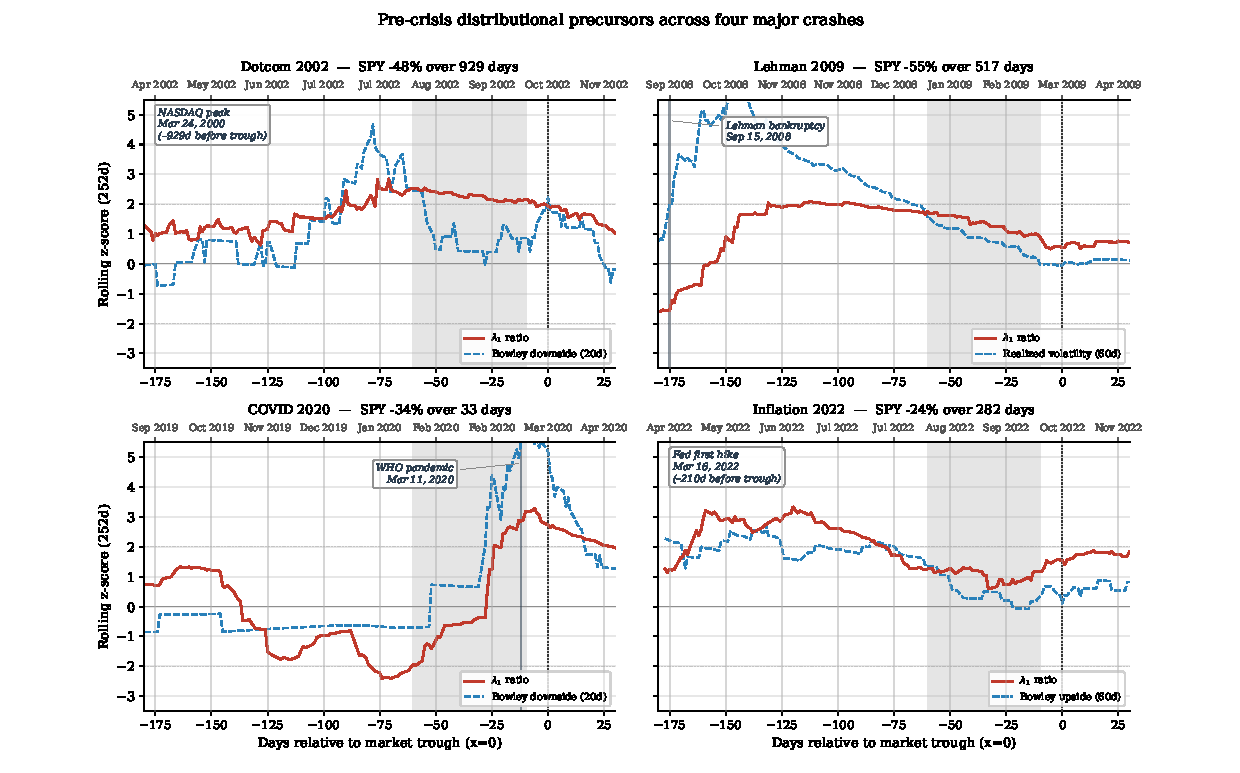
\includegraphics[width=\textwidth]{figure1_precursors.pdf}
  \caption{Pre-crisis distributional precursors across four major
  crashes. Each panel shows the rolling 252-day z-score of two
  distributional shape features in the 180 trading days preceding the
  market trough. The red solid line is the share of leading
  sector-eigenvalue energy ($\lambda_1$ ratio); the blue dashed line is
  the dominant crisis-specific shape descriptor: Bowley downside
  skewness for Dotcom and COVID, 60-day realised volatility for Lehman,
  60-day Bowley upside skewness for Inflation 2022. The shaded region
  marks the $-60$ to $-10$ trading-day window used for the effect-size
  analysis. Vertical lines and date labels indicate canonical event
  markers. Twin x-axes show calendar dates (top) and trading days
  relative to the market trough (bottom).}
  \label{fig:precursors}
\end{figure}

Three observations stand out. First, the share of leading
sector-eigenvalue energy ($\lambda_1$ ratio) is elevated in all three
slow-build cases for the better part of a year before the eventual
market trough. By the time price action makes the crisis obvious to a
casual observer, the cross-asset return covariance has already collapsed
toward a dominant common factor---sector-level diversification, the
diversification that buy-and-hold portfolios rely on, has been quietly
eroded. The signal is loud, sustained, and reproducible across crises
whose external causes---a technology bubble, a banking collapse, a
monetary tightening cycle---have nothing in common except their ultimate
destination.

Second, the dominant within-asset shape descriptor changes from crisis
to crisis. For Dotcom, downside skewness elongates as the cascading
sell-offs of the technology sector spill into the broader market. For
Lehman, 60-day realised volatility is already elevated months before the
trough---the Subprime crisis of 2007 had pre-conditioned the system, and
our framework registers this with a sustained volatility z-score above
$+3$ throughout the pre-crisis window. For Inflation 2022, the build-up
is gentler but no less persistent: Bowley upside skewness collapses as
the asymmetric optimism of the post-COVID rally drains out of the
market.

Third, when read across the four panels, the figure tells a
methodological story. No single feature captures all crisis types. The
slow-building structural crises require complementary descriptors---
eigenvalue concentration for the cross-asset structure, asymmetry and
tail descriptors for the within-asset distribution. The pipeline does
not insist on monolithic feature dominance; it relies instead on the
consistent presence of some deformation across multiple temporal scales,
and lets the specific feature mix vary with the crisis morphology.

\subsection{The numerical anatomy of pre-crisis stress}
\label{sec:anatomy}

To translate the visual observations of Figure~\ref{fig:precursors} into
quantitative claims, we computed Cohen's $d$ effect sizes between each
pre-crisis window (the 50 trading days from $-60$ to $-10$ relative to
the trough) and a calm baseline drawn from the pipeline's own stress
posterior. The baseline consists of all trading days for which the
aggregated stress posterior is at most 0.10 and which lie at least 90
days from any of the four crisis troughs (1{,}243 days in total).
Table~\ref{tab:cohend} reports these effect sizes for four feature
families.

The classical within-asset shape descriptors---realised volatility,
Bowley downside skewness, tail quantile---show effect sizes well above
2.9 in absolute value across all four crises. These are unusually strong
signals by conventional benchmarks (Cohen's $d > 0.8$ is ``large'').
But the most informative feature in the table is not the strongest; it
is the most cross-crisis robust. The sector-concentration ratio
$\lambda_1$ is the only feature with absolute Cohen's $d$ above 1.0
across all four crises, including the comparatively gentle Inflation 2022
build-up. Its magnitude is smaller than the within-asset descriptors, but
its consistency is unique: it is the only feature that does not collapse
on any single crisis. Figure~\ref{fig:separation} renders this
empirically.

% KORREKTUR 2: klarstellender Halbsatz zum Verhaeltnis der beiden
% Cohen's-d-Zahlen (Tabelle 1: min|d|=1.33 vs. Figure 2: gepoolt 2.23).
Note that Table~\ref{tab:cohend} reports the per-crisis
\emph{minimum} effect size ($\min|d| = 1.33$ for $\lambda_1$), a
deliberately conservative measure of cross-crisis robustness, whereas
the pooled effect size reported in Figure~\ref{fig:separation}
($d = +2.23$) aggregates all four pre-crisis windows into a single
comparison; the two numbers are consistent and answer different
questions.

\begin{table}[htbp]
  \centering
  \caption{Cohen's $d$ effect sizes between pre-crisis windows ($-60$ to
  $-10$ days before market trough) and a calm baseline (pipeline stress
  posterior $\le 0.10$, $\ge 90$ days from any crisis trough). Positive
  values indicate elevation during pre-crisis windows. The four feature
  families span different mathematical concepts: temporal volatility,
  distributional asymmetry, tail magnitude, and cross-asset structure.
  The minimum $|d|$ column reports the smallest absolute effect size
  across the four crises---a measure of cross-crisis robustness.}
  \label{tab:cohend}
  \begin{tabular}{llrrrrr}
    \toprule
    Feature family & Feature & Dotcom & Lehman & COVID & Inflation
      & $\min|d|$ \\
    \midrule
    Realised volatility   & rv\_20        & $+6.50$ & $+7.81$ & $+3.06$
      & $+3.58$ & 3.06 \\
    Bowley downside       & bow\_dn\_bg\_20 & $+8.31$ & $+8.62$ & $+3.33$
      & $+2.96$ & 2.96 \\
    Tail quantile         & q05\_20       & $-3.95$ & $-6.00$ & $-3.18$
      & $-2.90$ & 2.90 \\
    Sector concentration  & lambda1\_ratio & $+2.57$ & $+3.38$ & $+1.33$
      & $+1.84$ & 1.33 \\
    \bottomrule
  \end{tabular}
\end{table}

\subsection{The COVID anomaly: when the framework learns caution}
\label{sec:covid}

COVID is the structural outlier in our sample. The shock arrives from
outside the financial system entirely---a biological event, with no
precedent in the price-and-return record on which our pipeline is
trained. Three of the four crises in our test set follow the slow-build
morphology of Section~\ref{sec:chronic}; COVID does not. Its
distributional precursors emerge late, in the final 25 trading days
before the market trough, not in the months before. And here the
pipeline's behaviour deserves careful description.

The random-forest classifier registered elevated stress probability on
14 February 2020, five trading days before the SPY peak of 19 February.
Read in isolation, this would suggest pre-peak early warning. But the
particle filter, which integrates the classifier's signal through its
observation likelihood, did not cross the operational stress threshold
of 0.30 until 2 March 2020---twelve trading days after the peak, and
twenty-one trading days before the trough of 23 March. The sixteen-day
lag between the classifier signal and the filter confirmation is not a
defect. It is a feature.

The particle filter requires persistent distributional deformation
before committing posterior mass to a stress regime. This same
architectural property is what produces a false-positive rate of zero
during the 2017 low-volatility year---a year in which classical
momentum-based indicators generate frequent false alarms. The filter
trades pre-peak detection for calm-period discipline. For exogenous
shocks like COVID, this trade-off costs us the ability to claim pre-peak
detection; for endogenous build-ups like Dotcom, Lehman, and Inflation
2022, the same property protects us from the noise of normal market
turbulence. We therefore present the COVID episode not as a triumph of
pre-peak early warning, which the system does not claim and cannot
honestly claim, but as evidence of confirmation with substantial
lead-time before the eventual trough---a confirmation that arrived three
weeks before the market bottom, in a regime where pre-peak detection of
the underlying biological shock would have been informationally
impossible from financial data alone.

This is what we mean by authentic voice. Teiresias does not see what the
data cannot show. But he does speak---clearly and on time---when the
data begins to show it.

\begin{figure}[htbp]
  \centering
  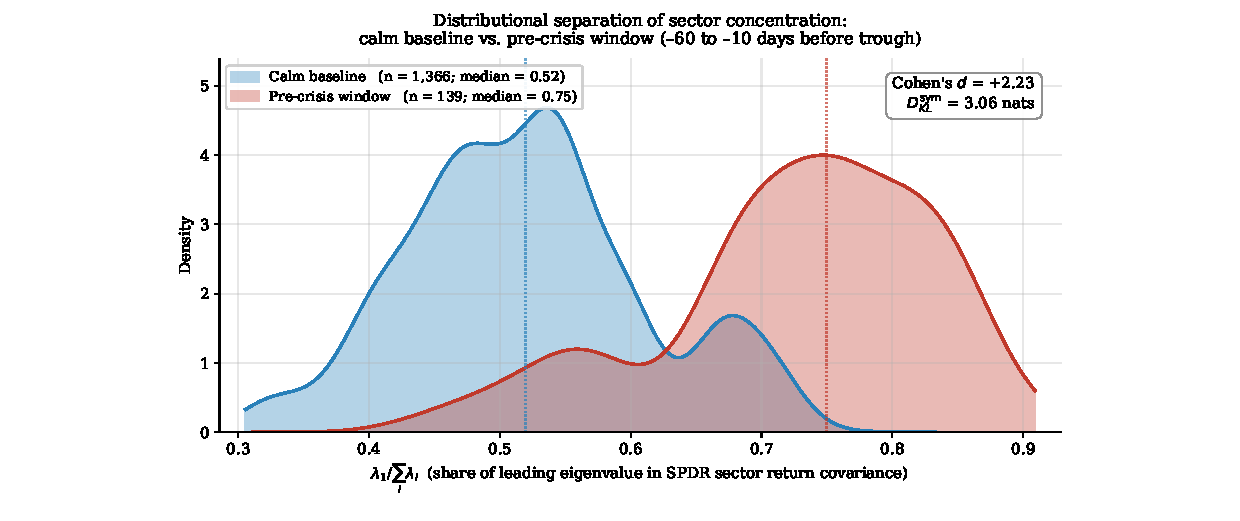
\includegraphics[width=0.92\textwidth]{figure2_separation.pdf}
  \caption{Distributional separation of the sector-concentration feature
  ($\lambda_1$ ratio) between calm baseline (blue) and pre-crisis
  windows (red, pooled across Dotcom 2002, Lehman 2009, COVID 2020, and
  Inflation 2022). Cohen's $d = +2.23$; symmetric Kullback-Leibler
  divergence $D^{\mathrm{sym}}_{KL} = 3.06$ nats. The pooled pre-crisis
  density is concentrated at higher values, consistent with the
  structural interpretation: sector-level diversification is reduced as
  the leading eigenvalue absorbs an increasing share of total
  cross-asset variance during the build-up to systemic stress.}
  \label{fig:separation}
\end{figure}

\subsection{Hormuz 2025: the art of staying calm}
\label{sec:hormuz}

Not every drawdown is a crisis. The Iran-Israel tensions of spring and
summer 2025, with their concerns about Hormuz Strait oil-supply
disruption, generated a peak-to-trough decline of approximately 19\% in
the S\&P~500---substantial, but bounded. Market commentary at the time
was sharply divided. One prominent strand projected systemic collapse---
a ``structural breakdown of the petrodollar system'' was one widely
circulated phrase. Another, equally prominent strand characterised the
episode as a measured repricing of geopolitical risk, accompanied by
unprecedented protective-options activity rather than panic selling.

Our framework's classification was Bear, not Crisis. The aggregated
stress posterior reached 1.000 during the relevant window---by the
numerical metric of Section~\ref{sec:oos}, the system ``detects''
Hormuz---but the posterior mass was concentrated on Bear states, with
the Crisis-regime probability bounded throughout. This classification
turned out to be consistent with the subsequent market evolution: a
recovery within two quarters, no cascade of liquidity stress, no
policy-grade intervention, no credit-spread blow-out of the kind that
characterises a true Crisis-regime episode.

What this case illustrates is something the binary literature on regime
detection often misses: the question of ``did the system detect the
event'' is less interesting than the question of ``did the system
correctly characterise the event.'' Our framework discriminates between
systemic panic and severe-but-bounded stress on the basis of how the
return distribution deforms across multiple temporal scales
simultaneously. The seven-regime taxonomy of Section~3.5 exists
precisely to make this distinction available; the Hormuz episode
demonstrates that the distinction is empirically meaningful and not
merely a notational convenience.

\subsection{Out-of-sample pipeline performance}
\label{sec:oos}

We close the section with the numerical summary that
quantitative-finance reviewers will look for first. On out-of-sample
data covering January 2015 through April 2026 (2{,}847 trading days),
the pipeline produces the following results.

For each of the three crises in the out-of-sample period---COVID 2020,
Inflation 2022, and Hormuz 2025---the aggregated stress posterior
reached its maximum within the 60 trading days preceding the market
trough: 0.998 for COVID, 0.999 for the inflation bear market of 2022,
and 1.000 for the Hormuz episode. Across the full test set, using a
stress-posterior threshold of 0.30 and a $\pm 90$ trading-day window
around each crisis trough as the positive class, the system achieves a
global true-positive rate of 77.4\% against a false-positive rate of
35.9\%. During the 2017 low-volatility year, used as a calm-period
stress test, the false-positive rate is 0.0\%.

A natural methodological question is whether the random-forest
classifier should be coupled more tightly to the particle filter---for
instance, through a convex combination
$L(r) = \lambda \cdot L_{kNN}(r) + (1-\lambda) \cdot L_{RF}(r)$ in the
spirit of \citet{Grisetti2007}. We tested this. Across
$\lambda \times T$ parameter sweeps spanning the natural range of
mixture weights and temperatures, the geometric $k$-NN likelihood proved
Pareto-dominant. We attribute this to a structural property: the
geometric likelihood expresses distance to the empirical core of each
regime in the standardised feature space, whereas the random-forest
posterior expresses confidence in regime identity. Mixing the two
confuses the inferential role of the filter, which is to integrate the
geometry over time rather than to repeat the classifier's instantaneous
judgement. We retain the random forest and Viterbi decoding as upstream
label generators, and the $k$-NN-based likelihood as the canonical
observation model. The mixing code remains in the companion repository
for reproducibility of this ablation.

Ten-seed hardening of the pipeline confirms bytewise reproducibility of
these numbers; the seeds and the snapshot are committed to the
repository.

% =====================================================================
\section{Conclusions}

This paper has proposed a particle filter framework for real-time regime
inference in financial markets, grounded in a methodological transfer
from probabilistic robotics and computer vision. The central
contribution is the integration of particle filtering with multi-scale
observation modelling: a multi-scale representation of the distributional
shape of return distributions, computed across a hierarchy of temporal
windows and transferred to the particle filter as a structured prior
through strategic injection.

The empirical validation rests on four major crisis episodes (Dotcom
2002, Lehman 2009, COVID 2020, Inflation 2022) and one differentiating
counter-case (Hormuz 2025). Across the four crashes, the share of
leading sector-eigenvalue energy ($\lambda_1$ ratio) is the only feature
in our analysis with cross-crisis robustness defined as $|d| > 1$ on
every episode; classical within-asset shape descriptors (realised
volatility, Bowley downside skewness, tail quantile) achieve
substantially larger effect sizes on most crises but vary more across
episodes. On the out-of-sample period 2015--2026, the pipeline produces
a global true-positive rate of 77.4\% against a false-positive rate of
35.9\%, with zero false positives during the 2017 low-volatility year.
For the abrupt COVID-19 shock, the particle filter confirmed the regime
transition twenty-one trading days before the market trough---a
confirmation-detector outcome we present as a feature of the system
rather than as evidence of pre-peak early warning.

The Hormuz episode of 2025 provides a different kind of validation. The
framework classified this period as Bear rather than Crisis, a
distinction reflecting a genuine structural difference in distributional
shape. The immunisation principle does not equate all severe drawdowns;
it discriminates between systemic panic and severe-but-bounded stress on
the basis of how the return distribution deforms across all temporal
scales simultaneously.

The results support the central claim: the richness of the observation
model and the structural informativeness of particle injection are the
primary enablers of early regime detection through this class of
methods. We therefore propose to direct research efforts towards the
construction and elaboration of a new class of indicators and
oscillators specifically designed for the early detection of regime
changes.

\subsection{Limitations}

The validation is conducted on a single index. The transition from
clusters to seven labelled regime categories involves a mapping step
that combines empirical cluster geometry with established market
terminology; the robustness of this mapping to alternative
cluster-to-regime assignments merits dedicated investigation in the
future. We focus on early detection of crash onset; early detection of
recovery and end-phase signals needs further work. The system does not
claim pre-peak detection of fully exogenous shocks, as discussed in
Section~\ref{sec:covid}; the COVID-19 case demonstrates confirmation
with substantial lead-time before the trough, not pre-peak detection.
The AUC-based scoring popular in regime-detection literature is not the
primary metric in our evaluation, which favours pre-peak posterior
magnitude and threshold-based binary classification with explicit
calm-period stress testing.

\subsection{Future Research Directions}

The contribution of this paper is intentionally framed as opening rather
than closing. We claim a central observation---that financial regime
transitions announce themselves through distributional deformation
across multiple temporal scales---and demonstrate that this observation
can be operationalised through particle-based inference with structurally
informed observation models. We do not claim a finished theory. The
instruments offered here are first instruments; the four directions
sketched below are not so much ambitions as invitations.

First, cross-asset generalisation: can regime detection transfer from
broad indices to individual assets? Which feature-relevance patterns
differ? Do single stocks require additional distributional descriptors
beyond the present feature set?

Second, sub-regime discrimination: can the framework detect corrections
and distinguish them from pullbacks in real-time? This is fundamentally
a binary classification task requiring finer distributional shape
analysis at the boundary between Sideways and Stress regimes.

Third, agricultural futures and commodity regime detection: how do
seasonal patterns interact with the multi-scale approach? Do
agricultural cycles require specialised temporal windows?

Fourth, and most fundamentally: the development of a new generation of
market indicators structurally sensitive to regime transitions, rather
than retrospective confirmations of them. How precisely can the onset of
a structural break be characterised, down to the resolution of
individual reversals?

Beyond refining existing models, a productive direction of research may
be to ask which aspects of market structure remain invisible to current
representations---and to investigate whether building new distributional
instruments might lead to better understanding of market regime
transitions.

% =====================================================================
\bibliography{references}

\end{document}
